\documentclass[a4paper]{book}
\usepackage{commeunjeustyle}

\begin{document}
\chapter*{Système d'équations linéaires}
% ressource http://univmaths.e-monsite.com/medias/files/cours-d-algebre-lineaire.pdf http://exo7.emath.fr/cours/ch_syslin.pdf
La résolution des systèmes d'équations linéaires appartient aux problèmes les plus anciens dans les mathématiques et ceux-ci apparaissent dans beaucoup de domaines, comme en traitement numérique du signal, en optimisation linéaire, ou dans l'approximation de problèmes non linéaires en analyse numérique
Les systèmes linéaires interviennent à travers leurs applications dans de nombreux contextes, car ils forment la base
calculatoire de l'algèbre linéaire. Ils permettent également de traiter une bonne partie de la théorie de l'algèbre linéaire
en dimension finie. C'est pourquoi ce cours commence avec une étude des équations linéaires et de leur résolution.
Le but de ce chapitre est essentiellement pratique : il s'agit de résoudre des systèmes linéaires. La partie théorique
sera revue et prouvée dans le chapitre « Matrices »
\section{Exemple introductif}
La somme des tailles d'un fils et du père est de 2,5 mètres. La différence de tailles  est de 0.5 mètres.
Quel est la taille du fils ? 
\subsection{Modélisation}
Soit la variable $x$ représentant la taille du fils et la variable $y$ représentant la taille du père.\\
La somme est 2,5 donc $x+y=2,5$.\\
La différence est 0,5 donc $y-x=0,5$.\\
Ainsi on cherche $x$ et $y$ vérifiant le système $(S)$  :
\begin{center}
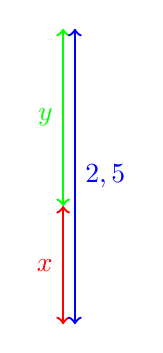
\begin{tikzpicture}[scale=1.5]
\draw[line width=0.3mm, <->,color=red] (0,0) -- node[left] {$x$}(0,1);
\draw[line width=0.3mm, <->,color=green] (0,1) -- node[left] {$y$}(0,2.5);
\draw[line width=0.3mm, <->,color=blue] (0.1,0) -- node[right] {$2,5$}(0.1,2.5);
\end{tikzpicture}
et
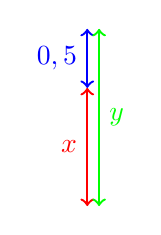
\begin{tikzpicture}[scale=1.5]
\draw[line width=0.3mm, <->,color=red] (0,0) -- node[left] {$x$}(0,1);
\draw[line width=0.3mm, <->,color=blue] (0,1) -- node[left] {$0,5$}(0,1.5);
\draw[line width=0.3mm, <->,color=green] (0.1,0) -- node[right] {$y$}(0.1,1.5);
\end{tikzpicture}
$\Leftrightarrow\quad \begin{cases}
{\color{red}x}+{\color{green}y}&={\color{blue}2,5}\\
{\color{red}x}+{\color{blue}0,5}&={\color{green}y}
\end{cases}\Leftrightarrow\quad \begin{cases}
{\color{red}x}+{\color{green}y}&={\color{blue}2,5}\\
{\color{red}-x}+{\color{green}y}&={\color{blue}0,5}
\end{cases}
$		
\end{center}


\subsection{Résolution par pivot de Gauss}
Pour déterminer l'ensemble des solutions $x$ et $y$ vérifiant ce système, une idée est de découpler par itérations les dépendances entre les inconnues dans les équations par combinaison ou élimination. A chaque itération, ces deux opérations transforment  un système d'équations en un autre équivalent (ayant les mêmes solutions).\\
L'application à l'exemple introductif est :
\begin{enumerate}
\item pour éliminer $x$ de la ligne 2,  on ajoute à la ligne 2 la ligne 1 :
$$\begin{cases}
x+y&=2,5\\
2y&=3
\end{cases}
$$
\item pour déterminer $y$, on divise la ligne 2 par 2 : 
$$\begin{cases}
x+y&=2,5\\
y&=1,5
\end{cases}
$$
\item pour éliminer $y$  de la ligne 2, on soustraie à la ligne 1 la ligne 2 :
$$\begin{cases}
x&=1\\
y&=1,5
\end{cases}
$$
\end{enumerate}
Ainsi l'ensemble des solution est l'unique solution $(1 , 1,5 )$ car ce dernier système d'équations est équivalent au premier.
\subsection{Structure de l'ensemble des solutions}
Le système équation :
$$(S)\quad \begin{cases}
x+y&=2,5\quad(D_1)\\
-x+y&=0,5\quad(D_2)
\end{cases}$$
est constitué de deux équations de deux droites $D_1$ et $D_2$. 
Trois cas se présentent alors :
\begin{enumerate}
\item Si les droites $D_1$ et $D_2$ ne sont pas parallèles, alors elle s'intersecte en un unique point et le système $(S)$ a une
unique solution.
\begin{center}
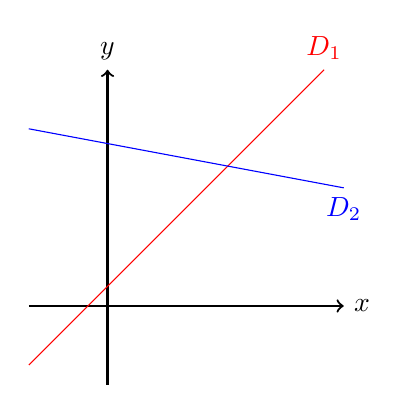
\begin{tikzpicture}[scale=0.5]
\draw[thick,->] (-2,0) -- (6,0)node[anchor=west] {$x$};
\draw[thick,->] (0,-2) -- (0,6)node[anchor=south] {$y$};
\draw[-,color=red] (-2,-1.5) -- (5.5,6)node[anchor=south] {$D_1$};
\draw[-,color=blue] (-2,4.5) -- (6,3)node[anchor=north] {$D_2$};
\end{tikzpicture}	
\end{center}
\item Si les droites $D_1$ et $D_2$  sont parallèles et non confondues, alors elle ne s'intersecte pas et le système $(S)$ n'a pas de solution.
\begin{center}
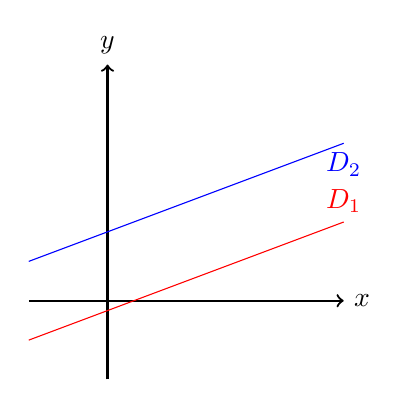
\begin{tikzpicture}[scale=0.5]
\draw[thick,->] (-2,0) -- (6,0)node[anchor=west] {$x$};
\draw[thick,->] (0,-2) -- (0,6)node[anchor=south] {$y$};
\draw[-,color=red] (-2,-1) -- (6,2)node[anchor=south] {$D_1$};
\draw[-,color=blue] (-2,1) -- (6,4)node[anchor=north] {$D_2$};
\end{tikzpicture}	
\end{center}
\item Si les droites $D_1$ et $D_2$  sont parallèles et  confondues, alors elle s'intersecte en une infinité de points et le système $(S)$ a une infinité de solutions.
\begin{center}
\begin{tikzpicture}[scale=0.5]
\draw[thick,->] (-2,0) -- (6,0)node[anchor=west] {$x$};
\draw[thick,->] (0,-2) -- (0,6)node[anchor=south] {$y$};
\draw[-,color=red] (-2,-1) -- (6,4)node[anchor=south] {$D_1=D_2$};
\end{tikzpicture}
\end{center}
\end{enumerate} 
Dans notre exemple, comme les vecteurs normaux aux deux droites $\begin{pmatrix}
1\\1
\end{pmatrix}$ et $\begin{pmatrix}
-1\\1
\end{pmatrix}$ ne sont pas colinéaires, les deux droites ne sont pas parallèles et donc admettent un unique point d'intersection.
\begin{center}
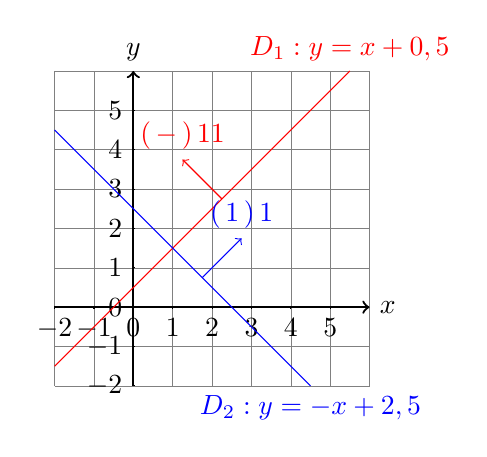
\begin{tikzpicture}[scale=0.5]
\draw[step=1cm,gray,very thin] (-2,-2) grid (6,6);
\draw[thick,->] (-2,0) -- (6,0)node[anchor=west] {$x$};
\draw[thick,->] (0,-2) -- (0,6)node[anchor=south] {$y$};
\foreach \x in {-2,-1,0,1,2,3,4,5}
   \draw (\x cm,1pt) -- (\x cm,-1pt) node[anchor=north] {$\x$};
\foreach \y in {-2,-1,0,1,2,3,4,5}
    \draw (1pt,\y cm) -- (-1pt,\y cm) node[anchor=east] {$\y$};
\draw[-,color=red] (-2,-1.5) -- (5.5,6)node[anchor=south] {$D_1 : y=x+0,5$};
\draw[-,color=blue] (-2,4.5) -- (4.5,-2)node[anchor=north] {$D_2 : y=-x+2,5$};

\draw[->,color=red] (2.25,2.75) -- (1.25,3.75)node[anchor=south] {$\begin{pmatrix}-1\\1\end{pmatrix}$};

\draw[->,color=blue] (1.75,0.75) -- (2.75,1.75)node[anchor=south] {$\begin{pmatrix}1\\1\end{pmatrix}$};
\end{tikzpicture}	
\end{center}
Ainsi l'ensemble des solution admet une unique solution.\\
La prochaine section est l'étude théorique qui permettra de généraliser à quelque soit le système d'équations linéaires
\begin{itemize}
\item la méthode de résolution à l'aide du pivot de gauss,
\item la structure de l'ensemble des résultats du système, c'est à dire  une unique solution ou bien aucune solution ou bien une infinité de solutions.
\end{itemize}


\section{Étude théorique}
\begin{Definition}[Équation linéaire]
On appelle \defi{équation linéaire} dans les variables  (ou inconnues) $x_1,\dots,x_n$ toute
relation de la forme
$$a_1 x_1 + \dots + a_n x_n = b $$
où $a_1,\dots ,a_n$ et $b$ sont des nombres réels.\\
\end{Definition}
\begin{Exemple}
$2x + 3y = 6$ est une équation linéaire, alors que les équations suivantes ne sont pas des équations
linéaires :
$2x + y^2 = 1$ ou $y = \sin x$.
\end{Exemple}



\begin{Definition}[Système d'équations linéaires]
Un \defi{système de $n$ équations linéaires à $p$ variables} est une liste de $n$ équations linéaires dans les variables  $x_1,\dots,x_p$.\\
La forme générale d'un système linéaire de $n$ équations à $p$ inconnues est la suivante :
$$\left\{{\begin{matrix}
a_{11}x_{1}&+&a_{12}x_{2}&+&\dots &+&a_{1p}x_{p}&=&b_{1}\\
a_{21}x_{1}&+&a_{22}x_{2}&+&\dots &+&a_{2p}x_{p}&=&b_{2}\\
\vdots&&\vdots&& &&\vdots&=&\vdots \\
a_{i1}x_{1}&+&a_{i2}x_{2}&+&\dots &+&a_{ip}x_{p}&=&b_{i}\\
\vdots&&\vdots&& &&\vdots&=&\vdots \\
a_{n1}x_{1}&+&a_{n2}x_{2}&+&\dots &+&a_{np}x_{n}&=&b_{n}\\
\end{matrix}}\right. $$
où  les nombres $a_{ij}$ sont les \defi{coefficients} du système et les nombres $b_i$ constituent le \defi{second membre} du système. Les coefficients $a_{ij}$ et $b_i$ donnés.\\
Le système est rangé 
\begin{itemize}
\item en \defi{lignes, $L_i$}, correspondant aux équations numérotées de $1$ à
$n$, 
\item en \defi{colonnes, $C_j$},  correspondant aux variables $x_j$
numérotées de $1$ à
$p$.
\end{itemize}
 La notation avec double indice $a_{i j}$ correspond à ce rangement : $i$ la ligne et  $j$ la colonne.
\end{Definition}
\begin{Exemple}
Le système suivant a $2$ équations et $3$ variables :
$$\left\{{\begin{matrix}
x_{1}&-&2x_{2}&+&4x_{3}&=&1\\
2x_{1}&+&1x_{2}&-&3x_{3}&=&2\\
\end{matrix}}\right. $$
\end{Exemple}
\begin{Definition}[Solution]
Une \defi{solution} du système linéaire est un p-uplet $(s_1,s2,\dots,s_p)$ tel que si l?on
substitue $s_1$ pour $x_1$
, $s_2$ pour $x_2$ et ainsi de suite  dans le système linéaire, on obtient une égalité.\\
 L'ensemble des solutions du système est l'ensemble de tous ces p-uplets.
\end{Definition}
\begin{Definition}[Implicite et explicite]
Un système d'équation linéaire est \defi{implicite} en décrivant une liste de 
de relations linéaires entre les variables. \\
\defi{Résoudre} un système signifie le rendre \defi{explicite} en déterminant l'ensemble des solutions du système.
\end{Definition}
\begin{Exemple}
Soit le système constitué de l'équation linéaire $3x_1 + x_2= 6$.\\ 
On paramètre $x_1$ avec $t$ puis on résolve l'équation par
rapport à $t$ : $x_1 = t$, $x_2 = -3t+6$.\\
La représentation paramétrique de l'ensemble des solutions du système est : 
$$\begin{pmatrix}
x_1\\x_2
\end{pmatrix}= t \begin{pmatrix}
1\\
-3
\end{pmatrix}+\begin{pmatrix}
0\\
6
\end{pmatrix},\quad \forall t\in \R.$$
Elle est explicite.
\end{Exemple}
 \begin{Definition}[Équation homogène]
Un \defi{système homogène} est un système ayant un second membre avec des coefficients nuls. Il est de la forme :
$$(S_H):\left\{{\begin{matrix}
a_{11}x_{1}&+&a_{12}x_{2}&+&\dots &+&a_{1p}x_{p}&=&0\\
a_{21}x_{1}&+&a_{22}x_{2}&+&\dots &+&a_{2p}x_{p}&=&0\\
\vdots&&\vdots&& &&\vdots&=&\vdots \\
a_{i1}x_{1}&+&a_{i2}x_{2}&+&\dots &+&a_{ip}x_{p}&=&0\\
\vdots&&\vdots&& &&\vdots&=&\vdots \\
a_{n1}x_{1}&+&a_{n2}x_{2}&+&\dots &+&a_{np}x_{n}&=&0\\
\end{matrix}}\right. $$
Le \defi{système homogène}, noté $S_H$, correspondant à un système $S$, est le même  excepté que les coefficients  du second membre ont été fixés à zéro.    
\end{Definition}
\begin{Exemple}
Le système homogène de ce système  
$\left\{{\begin{matrix}
x_{1}&-&2x_{2}&+&4x_{3}&=&1\\
2x_{1}&+&1x_{2}&-&3x_{3}&=&2\\
\end{matrix}}\right. $ est  $\left\{{\begin{matrix}
x_{1}&-&2x_{2}&+&4x_{3}&=&0\\
2x_{1}&+&1x_{2}&-&3x_{3}&=&0\\
\end{matrix}}\right. $.
\end{Exemple}
\begin{Theoreme}[Structure de l'ensemble des solutions d'un système linéaire]
Deux cas se présentent :
\begin{itemize}
\item ou bien le système n'admet pas de solution, on dit qu'il est \defi{incompatible}, 
\item ou bien le système admet au moins une solution $(x_1,\dots,x_n)$, appelée \defi{solution particulière}, on dit qu'il est \defi{compatible}. Dans ce cas, les solutions sont de la forme :
$$ S=\{\overbrace{(x_1,\dots ,x_n)}^{\text{Solution particulière}}+ \overbrace{(y_1,\dots,y_p)}^{\text{Solution homogène}}:\quad (y_1,\dots,y_p) \in S_H\}.$$
\end{itemize}
\end{Theoreme}
\begin{Demonstration}
Voir le chapitre sur les matrices.
\end{Demonstration}
\begin{Exemple}
Déterminer les solutions du système : 
$$\left\{{\begin{matrix}
x_{1}&-&2x_{2}&+&6x_{3}&=&1\\
2x_{1}&+&x_{2}&-&3x_{3}&=&2\\
\end{matrix}}\right. .$$
On a une solution particulière évidente $(1,0,0)$. L'équation homogène est :
$$\left\{{\begin{matrix}
x_{1}&-&2x_{2}&+&6x_{3}&=&0\\
2x_{1}&+&1x_{2}&-&3x_{3}&=&0\\
\end{matrix}}\right. .$$
En soustrayant deux fois la ligne 1 à la ligne 2, on obtient :
$$\left\{{\begin{matrix}
x_{1}&-&2x_{2}&+&6x_{3}&=&0\\
     &&5x_{2}&-&15x_{3}&=&0\\
\end{matrix}}\right. $$
En posant $x_3=t$, la ligne 2 donne $x_2=3t$ et la ligne 1 donne $x_1=0$. Ainsi l'ensemble des solutions du système est 
$$\{  \overbrace{(1,0,0)}^{\text{Sol particulière}} +\overbrace{t(0,3,1)}^{\text{Sol homogène}}:\quad\forall t \in \R \}.$$
\end{Exemple}
\section{Résolution par pivot de Gauss}
\begin{Definition}[Système équivalent]
On dit que deux systèmes linéaires sont \defi{équivalents} s'ils ont le même ensemble de solutions.
\end{Definition}

\begin{Definition}[Opérations élémentaires]
Les opérations suivantes sont appelées \defi{opérations élémentaires} sur le système :
\begin{enumerate}
\item  $L_i\leftrightarrow L_k$ : échanger deux lignes,
\item  $L_i\leftarrow \lambda L_i$ avec $\lambda\neq 0$ : multiplier une ligne par un nombre non nul, 
\item  $L_i \leftarrow  L_i +\lambda L_k$ avec $\lambda\in\R$ et $i\neq k$ : ajouter à la ligne $L_i$ $\lambda$ d'une autre ligne $L_k$.
\end{enumerate}
\end{Definition}

\begin{Proposition}[Équivalence par opérations élémentaires]
Les opérations élémentaires transforment un système linéaire en un système linéaire équivalent.
\end{Proposition}
\begin{Demonstration}
Voir le chapitre sur les matrices.
\end{Demonstration}
\begin{Remarque}
Pour résoudre un système, on utilisera une succession d'opérations élémentaires jusqu'à obtenir un système où l'on peut effecteur des substitutions.    
\end{Remarque}
\begin{Exemple}
Le système 
$\quad \begin{cases}
x+y&=\frac 5 2\\
-x+y&=\frac 1 2
\end{cases}
$
et le système 
$\begin{cases}
x+y&=\frac 5 2\\
2y&=3
\end{cases}
$ sont équivalents car le second système est la transformation du premier système par l'opération élémentaire $L_2\leftarrow L_2+L_1$. La ligne 2 du dernier système donne $y=\frac 3 2$ et substituant 
\end{Exemple}
\begin{Algorithme}[Pivot de Gauss]
Afin de faciliter la compréhension, nous noterons $\bigstar$ un pivot, $\blacksquare$ un coefficient non nul et 
$ $ un coefficient nul.\\
Par exemple, 
$\left\{{\begin{matrix}
0x_{1}&+&0x_{2}&+&1x_{3}&+&3x_{4}&=&2\\
0x_{1}&+&3x_{2}&+&0x_{3}&+&1x_{4}&=&1\\
0x_{1}&+&3x_{2}&+&1x_{3}&+&1x_{4}&=&3\\
\end{matrix}}\right.$ est noté $\left\{{\begin{matrix}
&+&&+&\blacksquare&+&\blacksquare&=&\blacksquare\\
&+&\blacksquare&+&\blacksquare&+&\blacksquare&=&\blacksquare\\
&+&\blacksquare&+&\blacksquare&+&\blacksquare&=&\blacksquare\\
\end{matrix}}\right.$

\begin{enumerate}
\item Identifier la colonne se trouvant le plus à gauche contenant au moins un élément non nul qui est le pivot.\\
Exemple : 
$$\left\{{\begin{matrix}
&+&&+&\blacksquare&+&\blacksquare&=&\blacksquare\\
&+&\blacksquare&+&\blacksquare&+&\blacksquare&=&\blacksquare\\
&+&\blacksquare&+&\blacksquare&+&\blacksquare&=&\blacksquare\\
\end{matrix}}\right.$$
Le pivot est sur la deuxième colonne et deuxième ligne. 
$$\left\{{\begin{matrix}
&+&&+&\blacksquare&+&\blacksquare&=&\blacksquare\\
&+&\bigstar&+&\blacksquare&+&\blacksquare&=&\blacksquare\\
&+&\blacksquare&+&\blacksquare&+&\blacksquare&=&\blacksquare\\
\end{matrix}}\right.$$
\item Permuter, s'il le faut, la première ligne avec une autre, pour que le coefficient en haut de la colonne soit non nul. C'est le pivot.\\
Exemple suite: 
$$\left\{{\begin{matrix}
&+&&+&\blacksquare&+&\blacksquare&=&\blacksquare\\
&+&\bigstar&+&\blacksquare&+&\blacksquare&=&\blacksquare\\
&+&\blacksquare&+&\blacksquare&+&\blacksquare&=&\blacksquare\\
\end{matrix}}\right.$$
On effectue $L_1\leftrightarrow L_2$
$$\left\{{\begin{matrix}
&+&\bigstar&+&\blacksquare&+&\blacksquare&=&\blacksquare\\
&+&&+&\blacksquare&+&\blacksquare&=&\blacksquare\\
&+&\blacksquare&+&\blacksquare&+&\blacksquare&=&\blacksquare\\
\end{matrix}}\right.$$
\item Ajouter des multiples adéquats de la première ligne aux lignes en-dessous pour annuler les
coefficients.\\
Exemple suite: 
$$\left\{{\begin{matrix}
&+&\bigstar&+&\blacksquare&+&\blacksquare&=&\blacksquare\\
&+&&+&\blacksquare&+&\blacksquare&=&\blacksquare\\
&+&\blacksquare&+&\blacksquare&+&\blacksquare&=&\blacksquare\\
\end{matrix}}\right.$$
On effectue $L_3\leftarrow L_3 -\lambda L_1$
$$\left\{{\begin{matrix}
&+&\bigstar&+&\blacksquare&+&\blacksquare&=&\blacksquare\\
&+&&+&\blacksquare&+&\blacksquare&=&\blacksquare\\
&+&&+&\blacksquare&+&\blacksquare&=&\blacksquare\\
\end{matrix}}\right.$$
\item Recommencer à l'étape (1) avec oubli de la première ligne.\\
Exemple suite: 
$$\left\{{\begin{matrix}
&+&\bigstar&+&\blacksquare&+&\blacksquare&=&\blacksquare\\
&+&&+&\blacksquare&+&\blacksquare&=&\blacksquare\\
&+&&+&\blacksquare&+&\blacksquare&=&\blacksquare\\
\end{matrix}}\right.$$
Le nouveau pivot est sur la troisième colonne et deuxième ligne
$$\left\{{\begin{matrix}
&+&\bigstar&+&\blacksquare&+&\blacksquare&=&\blacksquare\\
&+&&+&\bigstar&+&\blacksquare&=&\blacksquare\\
&+&&+&\blacksquare&+&\blacksquare&=&\blacksquare\\
\end{matrix}}\right.$$
Comme le nouveau pivot est déjà en haut de la colonne, on n'effectue rien à l'étape (2). Pour l'étape (3),  $L_3\leftarrow L_3 -\lambda L_2$
$$\left\{{\begin{matrix}
&+&\bigstar&+&\blacksquare&+&\blacksquare&=&\blacksquare\\
&+&&+&\bigstar&+&\blacksquare&=&\blacksquare\\
&+&&+&&+&\blacksquare&=&\blacksquare\\
\end{matrix}}\right. .$$ On recommence à l'étape (1) avec oubli des deux premières lignes. Le nouveau pivot est sur la dernière ligne et dernière colonne :
$$\left\{{\begin{matrix}
&+&\bigstar&+&\blacksquare&+&\blacksquare&=&\blacksquare\\
&+&&+&\bigstar&+&\blacksquare&=&\blacksquare\\
&+&&+&&+&\bigstar&=&\blacksquare\\
\end{matrix}}\right. .$$
La boucle se termine car chaque ligne contient un pivot.
\item Annuler tous les coefficients au dessus des pivots en commençant par la dernière ligne.\\
Exemple suite:  
$$\left\{{\begin{matrix}
&+&\bigstar&+&\blacksquare&+&\blacksquare&=&\blacksquare\\
&+&&+&\bigstar&+&\blacksquare&=&\blacksquare\\
&+&&+&&+&\bigstar&=&\blacksquare\\
\end{matrix}}\right. .$$
On effectue $L_2\leftarrow L_2 -\lambda L_3$ et $L_1\leftarrow L_1 -\mu L_3$
$$\left\{{\begin{matrix}
&+&\bigstar&+&\blacksquare&+&&=&\blacksquare\\
&+&&+&\bigstar&+&&=&\blacksquare\\
&+&&+&&+&\bigstar&=&\blacksquare\\
\end{matrix}}\right. .$$
et enfin $L_1\leftarrow L_1 -\lambda L_2$
$$\left\{{\begin{matrix}
&+&\bigstar&+&&+&&=&\blacksquare\\
&+&&+&\bigstar&+&&=&\blacksquare\\
&+&&+&&+&\bigstar&=&\blacksquare\\
\end{matrix}}\right. .$$
\item Exprimer les variables pivots en fonctions des variables paramétrées.\\
Exemple suite :\\  
Les variables des trois dernière colonnes exprimés en fonction de la variable de la première colonne.
\end{enumerate}
\end{Algorithme}
\begin{Exemple}[Unique solution]
\begin{center}
\begin{tabular}{c|c}
Système d'équations&	Opérations élémentaires	\\\hline
$\left\{\begin{matrix}2x_1&+&x_2&-&x_3&=&8&\\-3x_1&-&x_2&+&2x_3&=&-11&\\-2x_1&+&x_2&+&2x_3&=&-3&\end{matrix}\right.$&Pivot première ligne première colonne\\\hline
$\left\{\begin{matrix}2x_1&+&x_2&-&x_3&=&8&\\&&\frac 1 2x_2&+&\frac 1 2x_3&=&1&\\&&2x_2&+&1x_3&=&5&\end{matrix}\right.$&$\left.\begin{matrix}\\L_2\leftarrow L_2-\frac 3 2 L_1\\ L_3\leftarrow L_3+ L_1 \end{matrix}\right.$\\\hline
$\left\{\begin{matrix}2x_1&+&x_2&-&x_3&=&8&\\&&\frac 1 2x_2&+&\frac 1 2x_3&=&1&\\&&&&-x_3&=&1&\end{matrix}\right.$&$\left.\begin{matrix}\\\\ L_3\leftarrow L_3-4 L_2 \end{matrix}\right.$\\\hline
$\left\{\begin{matrix}2x_1&+&x_2&-&x_3&=&8&\\&&\frac 1 2x_2&+&\frac 1 2x_3&=&1&\\&&2x_2&+&1x_3&=&5&\end{matrix}\right.$&$\left.\begin{matrix}\\L_2\leftarrow L_2-\frac 3 2 L_1\\ L_3\leftarrow L_3+ L_1 \end{matrix}\right.$\\\hline
$\left\{\begin{matrix}2x_1&+&x_2&&&=&7&\\&&\frac 1 2x_2&&&=&\frac 3 2&\\&&&&-x_3&=&1&\end{matrix}\right.$&$\left.\begin{matrix}L_1\leftarrow L_1- L_3\\L_2\leftarrow L_2+\frac 1 2 L_3\\  \end{matrix}\right.$\\\hline
$\left\{\begin{matrix}2x_1&&&&&=&4&\\&&\frac 1 2x_2&&&=&\frac 3 2&\\&&&&-x_3&=&1&\end{matrix}\right.$&$\left.\begin{matrix}L_1\leftarrow L_1- 2L_2\\\\  \end{matrix}\right.$\\\hline
$\left\{\begin{matrix}x_1&&&&&=&2&\\&&x_2&&&=&3 &\\&&&&x_3&=&-1&\end{matrix}\right.$&$\left.\begin{matrix}L_1\leftarrow L_1- 2L_2\\\\  \end{matrix}\right.$\\\hline
\end{tabular}
\end{center}
L'ensemble des solution est l'unique triplet $(2,3,-1)$.
\end{Exemple}
\begin{Exemple}[Une infinité de solutions]
 Considérons le système homogène
$$\left\{\begin{matrix}
3x_1 &+& 3x_2 &-& 2x_3   & &      &-& x_5 &= 0\\
-x_1 &-& x_2  &+& x_3  &+& 3x_4 &+& x_5 &= 0\\
2x_1 &+& 2x_2 &-& x_3 &+& 2x_4 &+& 2x_5 &= 0\\
     &&       & & x_3 &+& 8x_4 &+& 4x_5 &= 0
     \end{matrix}
\right.$$
L'application de l'algorithme du pivot de Gauss donne le système équivalent suivant :
$$\left\{\begin{matrix}
x_1 &+& x_2 &&    & &      &+& 13x_5 &= 0\\
 -&  &+& x_2 &&  &+& 20x_5 &= 0\\
 &&  && && x_4 &-& x_5 &= 0\\
     &&       & & x_3 &+& 8x_4 &+& 4x_5 &= 0
     \end{matrix}
\right.$$
Les variables pivots sont $x_1$, $x_3$ et $x_4$ alors que les variables paramétrées sont $x_2$ et $x_5$. Posons alors
$x_2 = s$ et  $x_5 = t$.
On obtient
$$\left\{\begin{matrix}
x_1 &=& -s &-13t\\
x_2 &=& s&\\
x_3 &=&&-20t\\
x_4&=&&2t\\
x_5 &=& &t
\end{matrix}
\right.$$
L'ensemble des solutions est donc
$$S=\{s(-1,1,0,0,0)+t(-13,0,-20,2,1):\forall s,y\in\R\}.$$
\end{Exemple}

\begin{Exemple}[Pas de solutions]
 Considérons le système homogène
$$\left\{\begin{matrix}
x_1 &+& x_2  &= 1\\
x_1 &-& x_2  &= 1\\
x_1 &-& 2x_2 &=2
     \end{matrix}
\right.$$
L'application de l'algorithme du pivot de Gauss ($L_2\leftarrow L_2-L_1$ et $L_3\leftarrow L_3-L_1$) donne le système équivalent suivant :
$$\left\{\begin{matrix}
x_1 &+& x_2  &= 1\\
 &-& 2x_2  &= 0\\
 &-& 3x_2 &=1
     \end{matrix}
\right.$$
Comme $x_2$ doit être égale à $0$ et à $-\frac 3 2$, il n'existe pas de solution au système.
\end{Exemple}
\end{document}
